\section{Аннотация}
Мы живем в очень интересное время. Время, когда у практически у каждого есть мобильный телефон в кармане, персональный компьютер на рабочем столе, телевизор на кухне и практически неограниченное «облачное» хранилище информации. Время, когда со всех сторон нас окружают машины. А что же превращает эти машины из груды железа в вещи, к которым мы так привыкли? \\
Эту важную роль на себя берет программное обеспечение. ПО играет роль души, которая делает разнообразные устройства так близки нам. \\
Для того что бы сделать программное обеспечение наиболее удачным, нужен хороший инструмент. Инструментом для создания ПО является язык программирования. \\
На сайте The Language List\footnote{Киннерсли Б. ``Language List'' официальный сайт Канзаского университета URL:http://people.ku.edu/~nkinners/LangList/Extras/langlist.htm дата обращения: 18.09.2012}  
сейчас представлено около 2500 языков, но сколько из них реально используется и почему только несколько их них получили широкое распространение в среде программистов? \\
В нашей работе мы поставили цель, выяснить какие факторы привели к появлению и распространению современных наиболее популярных и интересных нам языков программирования. \\
Для достижения цели нужно ответить на вопросы: как развивались языки программирования, какие области программного обеспечения они охватывали, какие парадигмы программирования поддерживали и какие факторы повлияли на популяризацию данного языка программирования. Для ответов на данный вопрос нужно решить следующие задачи. Первое, какие языки имеют наибольший успех среди программистов. Второе, составить хронологическую модель развития языков. 
И третье рассмотреть каждый язык в отдельности, выделить его основные характеристики и определить факторы, из-за которых он получил свою  репутацию.
\section{Рейтинги популярности языков программирования.}
Существует множество рейтингов и способов оценки языков программирования. Мы в своей работе рассмотрим три из них:\\
ohloh.net Language Comparison\\
TIOBE Programming Community Index\\
The RedMonk Programming Language Rankings\\
\subsection{TIOBE Programming Community Index}
http://www.tiobe.com/index.php/content/company/GeneralInfo.html\\
Компания TIOBE занимается оценкой качества программных систем на основе оценки этих систем на соответствие своим стандартам программирования. \\
http://www.tiobe.com/index.php/content/paperinfo/tpci/tpci\_definition.htm\\
Для попадания в рейтинге TIOBE язык программирования должен отвечать двум требованиям:\\
На википедии должна быть страничка посвященная этому языку.\\
Язык программирования должен быть полным по Тьюрингу. Соответсвенно такие языки как HTML, XML, SQL не учитываются данным рейтингом.
Но различные расширения языка SQL, например PL/SQL, входят в рейтинг.\\
Рейтинг расчитывается на основе подсчета количества результатов в выдаче поисковых систем при запросе "<называние языка> programming". 
Данное число домножается на специальный коэффициент, установленный для каждой
 используемой поисковой системы:
 
    Google: 30\%\\
    Blogger: 30\%\\
    Wikipedia: 15\%\\
    YouTube: 9\%\\
    Baidu: 6\%\\
    Yahoo!: 3\%\\
    Bing: 3\%\\
    Amazon: 3\%\\
Количество результатов в выдаче определяет рейтинг языка. Рейтинги нормализуются по сумме первых пятидесяти языков. Т.о. первые 50 языков в сумме будут иметь рейтинг 100\%.
После для каждого результата подсчитывается количество ложных совпадений, таких как выдачи по запросу "Basic programming" страницы "Improve your basic programming skills in Java".
Подсчитывается процент таких промахов для первых ста страниц выдачи, дальше этот процент вычитается из общего количества результатов. \\
Так же вычисляются статусы языков на основе изменния их рейтинга, но нас это мало волнует.\\
http://www.tiobe.com/index.php/content/paperinfo/tpci/index.html
\begin{enumerate}
\item c 
\item Java
\item Objective-c
\item c++
\item c\#
\item PHP
\item (Visual)Basic
\item Python
\item Perl
\item JavaScript
\end{enumerate}
\subsection{ohloh.net Language Comparison Page}
Ohloh --- публичный ресурс посвященный свободному и открытому программному обеспечению. Он предоставляет возможности для общения разработчиков, аналитику и поиск по проектам. 
http://meta.ohloh.net/us/
На странице проекта можно вывести и просмотреть график отражающий популярность языков.
График показывает результаты для языков выбранных пользователем. Значения на графике --- это сумма все коммитов за месяц, которые содержат хотя бы одну строчку на 
запрашиваемом языке. Если в коммите несколько языков, то он защитывается в пользу всех. Информация собирается уже более 20 лет, и не включает текущий месяц, т.к. он еще не закончился.\\
meta.ohloh.net/compare\_languages/
самые популярные языки\\
\begin{enumerate}
\item c
\item java
\item c++
\item python
\item javascript
\item php
\item ruby
\item c\#
\item perl
\item objective-c
\end{enumerate}
я специально исключил неполные по тьюрингу языки (html, sql, css) чтобы добиться соответствия результатам различных рейтингов.

\subsection{The RedMonk Programming Language Rankings}
http://redmonk.com/\\
http://redmonk.com/about/\\
RedMonk --- аналитическая компания сфокусированная на разработчиках.????????????????????????????????\\
http://redmonk.com/sogrady/2012/02/08/language-rankings-2-2012/\\
Их методика составления рейтинга весьма и весьма проста, впервые она была предложена Дрю Конвеем (Drew Conway) 
(http://www.dataists.com/2010/12/ranking-the-popularity-of-programming-langauges/) в 2010 году. С тех пор уже второй год компания RedMonk 
обновляет статистику.\\
рейтинг предствляет из себя график осями которого является: популярность на GitHub  и популярность на Stack Overflow.
Для расчета популярности на Stack Overflow ведется подсчет тэгов. А на GitHub есть свой собственная система подсчета количества проектов на каждом из языков.\\
В результате получается картинка:	

\begin{figure}[H]
\center{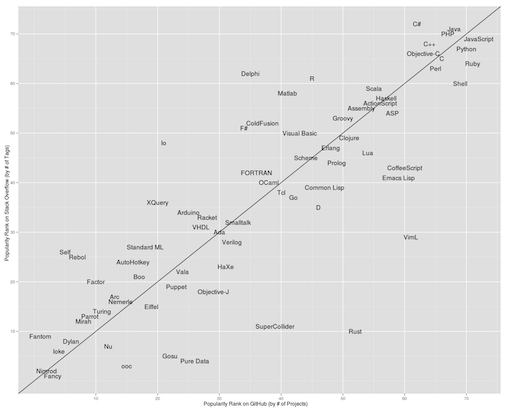
\includegraphics{image/redmonk.png}}
\caption{The RedMonk Programming Language Rankings.}
\label{ris:redmonk}
\end{figure}
Т.к. график двумерный, то нельзя однозначно решить какой из языков лучше. Поэтому просто выберем языки входящие в правую верхнюю группу. 
\begin{itemize}
\item C\#
\item Java
\item JavaScript
\item C
\item C++
\item Perl
\item Python
\item Ruby
\item Objective-C
\item PHP
\end{itemize}
\subsection{Выбор популярных языков}
Можно заметить, что не смотря на выбор рейтинга популярные языки программирования везде остаются примерно одни и те же лишь меняя своё место. 
Так что самыми популярными можно назвать:
\begin{itemize}
\item C
\item Java
\item С++
\item С\#
\item Objective-C
\item JavaScript
\item Python
\item Ruby
\item Perl
\item PHP
\end{itemize}

\section{Раняя история языков программирования.}
Програмиирование как явление появилось за долго до появления ЭВМ.\\
Первым в истории программируемым устройством стал ткацкий станок Жаккарда.\\
\\
Computers: The Life Story Of A Technology\\
 Авторы: Eric Gottfrid Swedin,David L. Ferro\\
 http://books.google.ru/books?id=c1QbNtTz4CYC\&pg=PA15\&hl=ru\&source=gbs\_selected\_pages\&cad=3\#v=onepage\&q\&f=false\\
\\
Француз Жозеф Мари Жаккард (1752-1834) изобрел первую программируемую машину с циклами в 1801 году. Эта машина не использовалась для вычислений. 
Это был ткацкий станок для узорчатых материй. Узор задавался при помощи набора перфокарт. Первым перфокарты для ткацких станков применил 
Jacques de Vaucanson (1709-1782) в 1745 году, но его машине нужно было скармливать карты по одной за раз. Станок Жаккарда в свою очередь
мог выполнять циклы из заранее установленных перфокарт, создавая повторяющийся узор. В конечном итоге была создана колода из 24000 карт.\\
Машина Бэббиджа\\
????????????????????????????????????????????????????????????????????????????\\
??????????????????????????????????????????????????????????????????????????\\
Программы загружались в неё при помощи жаккардовских первокарт. \\
Бэббидж предусмотрел подсоединение к своей машине нескольких считывателей перфокарт. Причем некоторые из них могли контролировать работу других. 
Причем можно было как пропускать несколько карт, так и считывать карты в обратном порядке. Это позволяло пропускать или повторять участки программы, что
уже соответсвовало трем основным типам выражений: последовательный, итеративыный и условный. \\
????????????????????????????????????????????\\
машина так и не была создана при жизни и вот только недавно...
?????????????????????????????????????????\\
http://ieeexplore.ieee.org/xpl/articleDetails.jsp?arnumber=1253887\\
@article{Fuegi:2003:LBC:1435605.1436041,
 author = {Fuegi, John and Francis, Jo},
 title = {Lovelace \& Babbage and the Creation of the 1843 'Notes'},
 journal = {IEEE Ann. Hist. Comput.},
 issue_date = {October 2003},
 volume = {25},
 number = {4},
 month = oct,
 year = {2003},
 issn = {1058-6180},
 pages = {16--26},
 numpages = {11},
 url = {http://dx.doi.org/10.1109/MAHC.2003.1253887},
 doi = {10.1109/MAHC.2003.1253887},
 acmid = {1436041},
 publisher = {IEEE Educational Activities Department},
 address = {Piscataway, NJ, USA},
} 

Ада Лавлейс, дочь лорда Байрона, перевела и дополнила комментариями труд «Sketch of the Analytical Engine». 
Её имя часто ассоциируют с именем Бэббиджа. Утверждается также, что она является первым программистом, 
хотя это утверждение и значение её вклада многими оспаривается.\\
 ????????????????????????????????????????????????????????\\
\section{История C.}